\documentclass[FCD_GNN.tex]{subfiles}

\begin{document}
\chapter{Implementation}
\label{chapter:Implementation}

This chapter describes the main implementation settings used for training the
proposed model.
It outlines the key characteristics of the hardware on which the experiments
were conducted and presents the web interface developed to facilitate
interaction with the different model variants.


\section{Training Settings}
In this work, we aim to follow the training protocol of the MELD authors to
ensure a fair and consistent comparison.
The proposed framework was trained using the following hyperparameters.
 
The training batch size was fixed at 8 and the validation batch size at 4. 
The initial learning rate was set to $3 \times 10^{-4}$ and optimized using 
the OneCycleLR scheduler (maximum learning rate $3 \times 10^{-3}$). 
The schedule included a warm-up phase during the first 10\% of training steps, 
followed by cosine annealing. 
Training was performed for up to 100~epochs (minimum 20~epochs), 
with early stopping applied if the validation performance did not improve for 20~epochs.  
For evaluation, we trained an ensemble of five independently initialized models (seeds 42–46). 
At test time, we averaged their per-vertex predictions to form the final output.  

The model integrated surface-based graph features and contextual text embeddings. 
Feature channel dimensions across the encoder stages were
$[32,32,64,64,128,128,256]$, 
with corresponding text sequence lengths
$[128,64,64,32,32,16,16]$, 
and a maximum text length of 256~tokens. 
Deep supervision was employed with levels 
$I_{ds} = [6,5,4,3,2,1]$ 
and associated weights \\
$w_{ds} = [0.5, 0.25, 0.125, 0.0625, 0.03125, 0.0150765]$~\cite{Ripart2025MELD}. 
The text encoder was initialized from RadBERT, 
with a projection dimension of 768.  

To address class imbalances, non-lesional hemispheres were undersampled, 
ensuring that approximately one third of training examples contained a lesion. 
Data augmentation strategies included: 

\begin{table}[H]
\centering
\caption{Data augmentation strategies applied during training~\cite{Ripart2025MELD}.}
\begin{tabular}{ll}
    \toprule
    \textbf{Transformation} & \textbf{Probability} \\
    \midrule
    Random flipping & 0.5 \\
    Gaussian blur & 0.2 \\
    Spinning & 0.2 \\
    Warping & 0.2 \\
    Brightness/contrast/gamma & 0.15 each \\
    Gaussian noise & 0.15 \\
    Low-resolution simulation & 0.25 \\
    \bottomrule
\end{tabular}
\end{table}
    
\subsection*{Hardware} 
All experiments were performed on the \emph{Bender} high-performance computing cluster at the University of Bonn, 
equipped with NVIDIA A100 GPUs (80~GiB each) and AMD EPYC CPUs. 

A detailed description of the system can be found in the official documentation\footnote{\url{https://www.hpc.uni-bonn.de/en/systems/bender}}. 
Our implementation used PyTorch~2.1.0+cu121, TorchVision~0.16.0+cu121, TorchAudio~2.1.0+cu121, Torch Geometric~2.5.3, Torch Scatter~2.1.2, 
TorchMetrics~0.11.4, and Python~3.9.18. 

To ensure reproducibility, a complete software environment has been provided via Docker.
The corresponding Dockerfiles and installation instructions are available in our GitHub repository\footnote{\url{https://github.com/Wektor607/FCD-Detection/tree/docker-inference-fix/meld_graph}}.

\section{Web Interface}
To make it easier to use different pretrained models, we developed a web interface that offers an accessible and intuitive way for users to interact with the lesion detection system.

\begin{figure}[H]
    \centering
    \includegraphics[width=0.8\textwidth]{pictures/photo_1.png}
    \caption{Main page of the web interface with a brief project description and navigation buttons.}
\end{figure}

The main page presents a brief overview of the project and includes navigation controls that let users explore the documentation or move on to the prediction page for processing a specific patient.

\begin{figure}[H]
    \centering
    \includegraphics[width=0.8\textwidth]{pictures/photo_2.png}
    \caption{Upload page where the user selects a model, adds a description, and uploads an HDF5 file for analysis. 
    \textit{Note: the current prototype accepts only a single HDF5 file.}}

\end{figure}

The workflow begins on the upload page, where the user selects one of the trained models, optionally adds a short textual description, and uploads an HDF5 file for analysis. The current prototype supports the upload of a single HDF5 file at a time.

\begin{figure}[H]
    \centering
    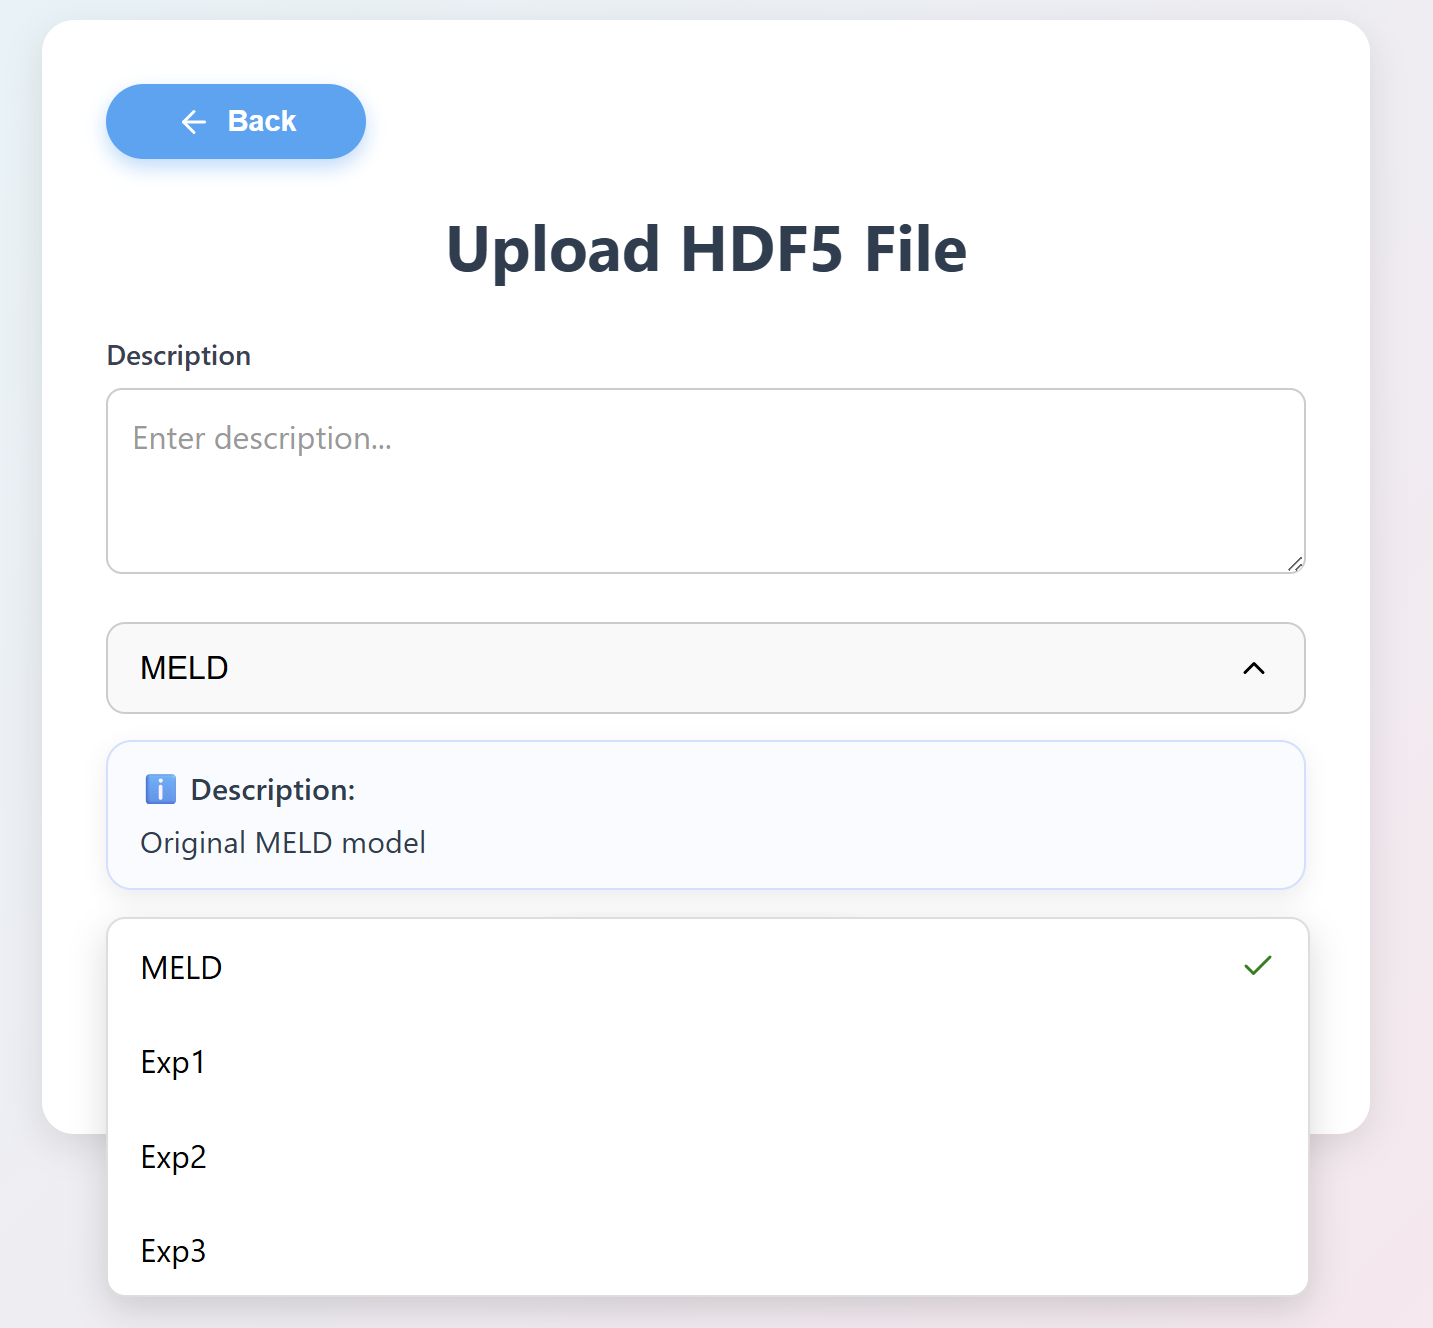
\includegraphics[width=0.6\textwidth]{pictures/photo_3.png}
    \caption{Dropdown menu for selecting among trained models.}

\end{figure}

To support different use cases and experimental settings, the interface includes a model selection menu listing all available trained variants. 
These include the baseline MELD model, two vision-only architectures (\texttt{Vision--only} and \texttt{Vision--only+SA}) with minor architectural differences, and the multimodal \texttt{Vision+LM} model trained on various textual inputs. 
Each option is accompanied by a short explanation, similar in style to modern LM model pickers, helping users choose between faster or more accurate configurations.

\begin{figure}[H]
    \centering
    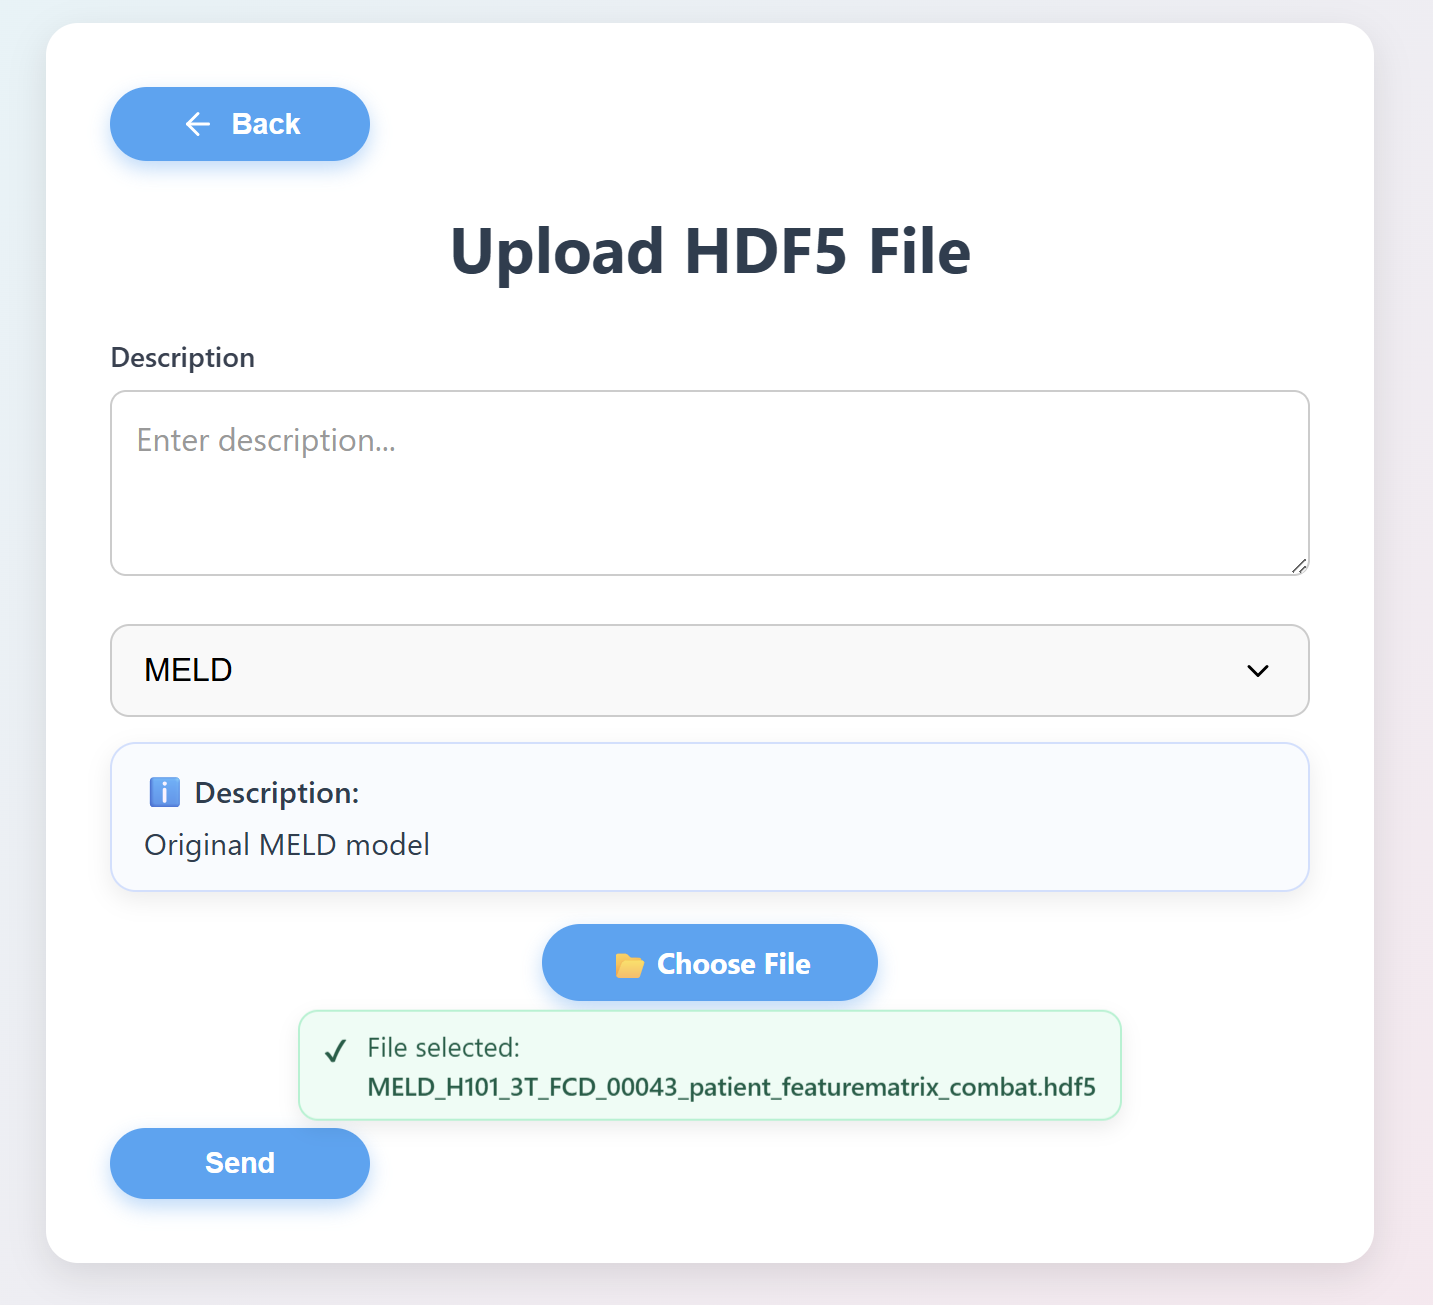
\includegraphics[width=0.6\textwidth]{pictures/photo_4.png}
    \caption{Example of a successfully uploaded file ready for processing.}
\end{figure}

Once a file is uploaded successfully, the interface confirms that the case is ready for processing and allows the user to initiate inference.
After the prediction is complete, the results page provides two complementary views of the output:
\begin{enumerate}[label=(\roman*)]
\item representative 2D MRI slices with the predicted lesion regions overlaid for quick inspection, and
\item a 3D cortical surface visualization rendered for both hemispheres (left and right), shown from two complementary viewpoints (anterior and posterior) to improve interpretability and spatial understanding.
\end{enumerate}

\begin{figure}[H]
    \centering
    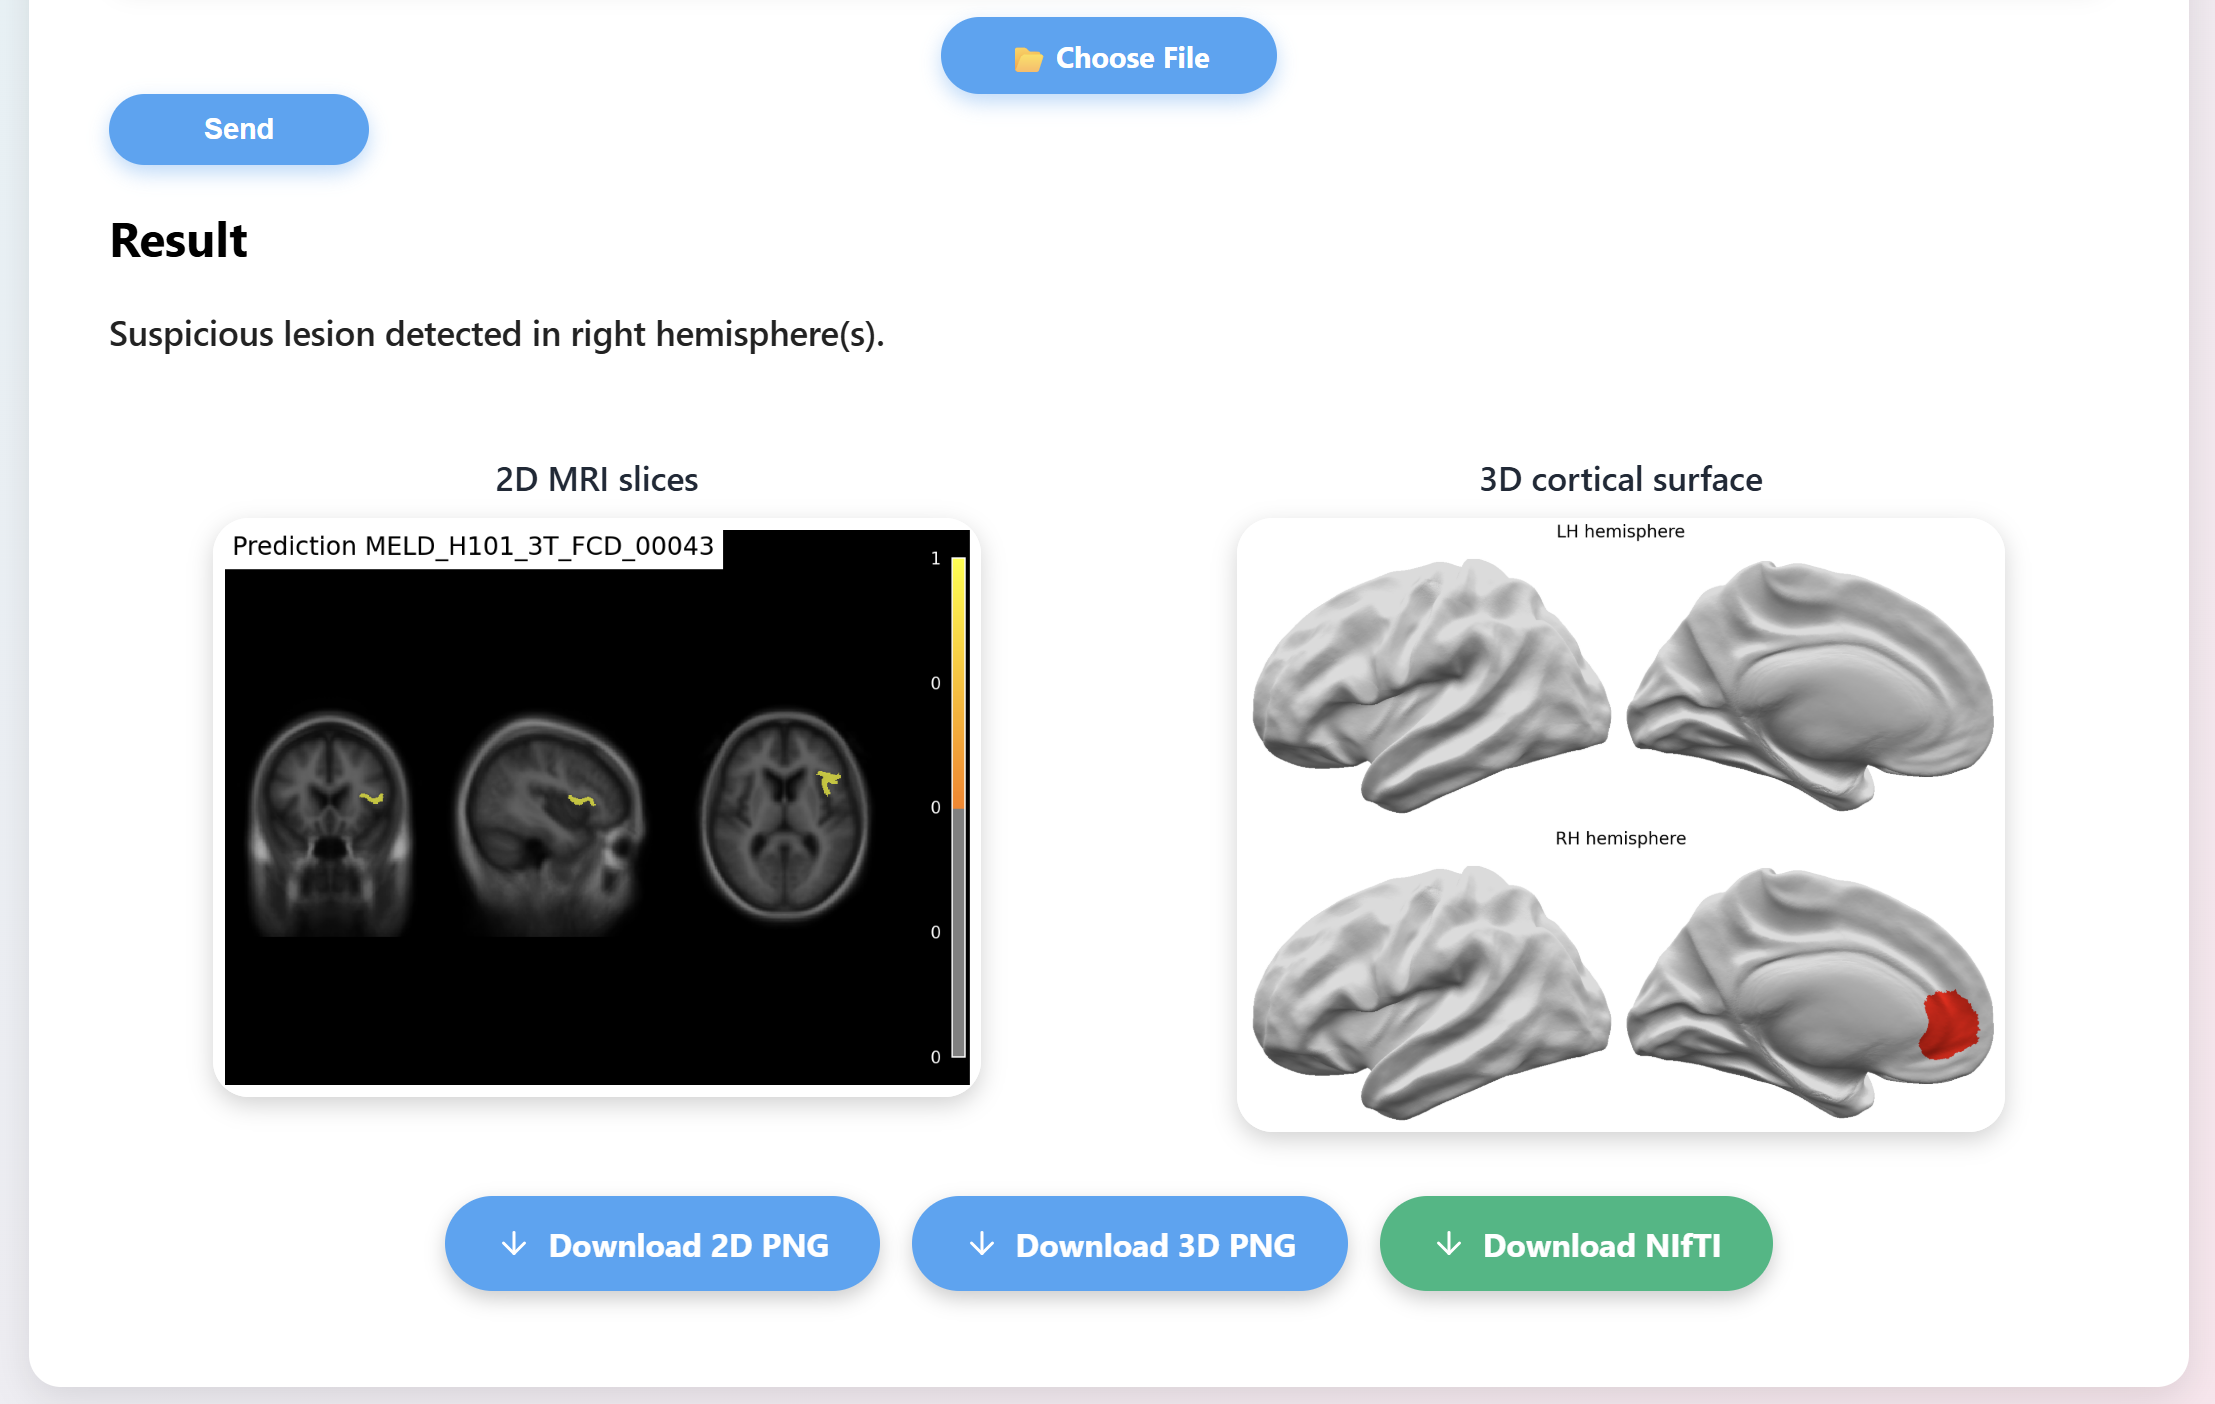
\includegraphics[width=0.6\textwidth]{pictures/photo_5.png}
    \caption{Web interface showing the inference output: 2D MRI slice overlays and a 3D cortical surface rendering for both hemispheres (LH/RH) from complementary viewpoints (anterior/posterior). All outputs can be exported as PNG (2D/3D) and as a NIfTI volume for further analysis in 3D medical imaging tools.}
    \label{fig:web_inference_result}
\end{figure}

All generated visualizations can be downloaded as PNG files (2D slices and 3D renderings), and the full volumetric prediction is additionally provided in NIfTI format for further analysis in standard 3D medical imaging software.
This design supports both general users (rapid visual validation) and developers/researchers (downstream processing and quantitative evaluation).

\end{document}